\subsection{1D exact}

\begin{frame}{1D: Transverse Field Ising}

    \begin{minipage}{.75\textwidth}

        \begin{figure}
            \center
            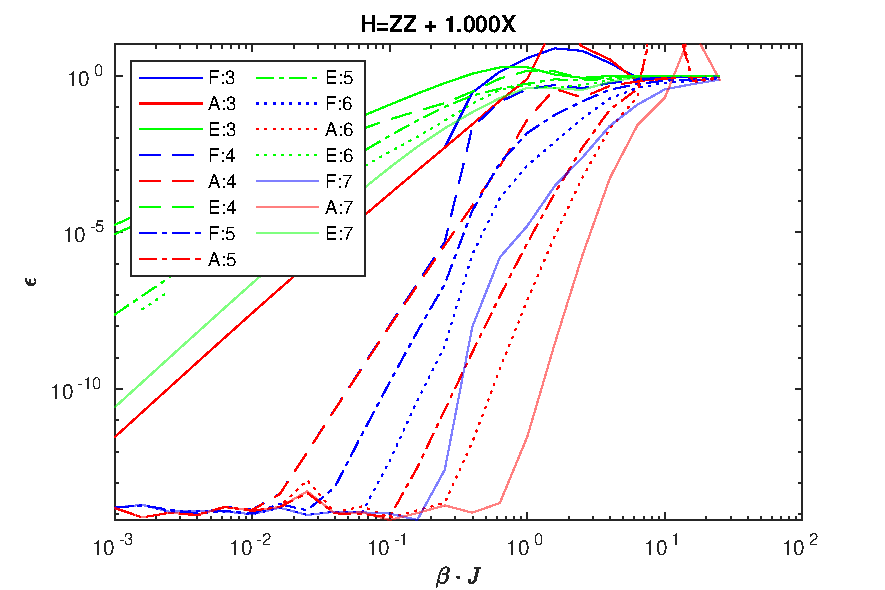
\includegraphics[width=\textwidth]{../Figuren/benchmarking/t_ising.pdf}
        \end{figure}

    \end{minipage}
    \begin{minipage}{.14\textwidth}
        \begin{table}[]
            \caption{$\chi$}
            \begin{tabular}{l|l l }
                  & A  & E/F \\
                \hline
                3 & 5  & 10  \\
                5 & 21 & 42  \\
                7 & 85 & 170 \\
            \end{tabular}
        \end{table}
    \end{minipage}

\end{frame}

\begin{frame}{1D: Heisenberg XXX}

    \begin{figure}
        \center
        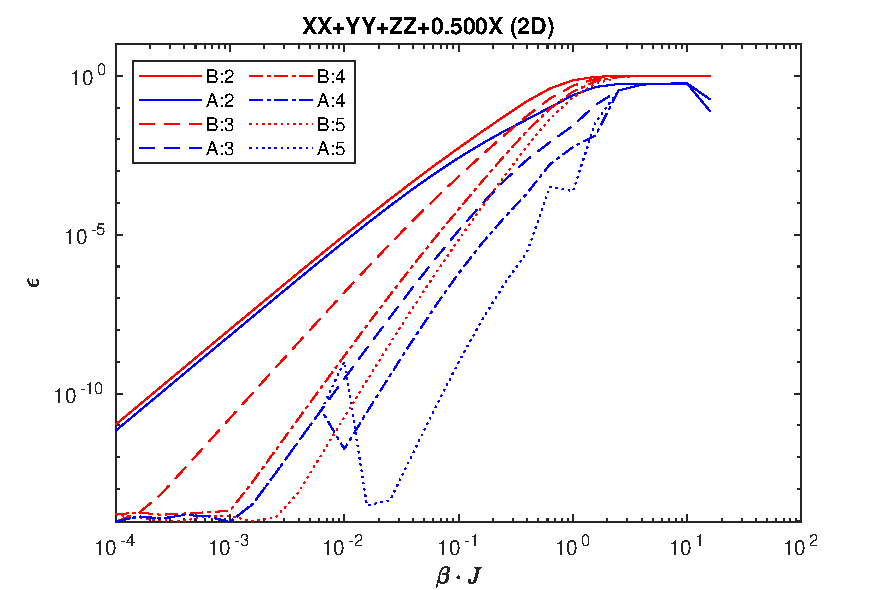
\includegraphics[width=0.75\textwidth]{../Figuren/benchmarking/t_heis_XXX.pdf}
    \end{figure}

\end{frame}

\subsection{2D exact}

\begin{frame}{2D: TFI}

    \begin{minipage}{.75\textwidth}
        \begin{figure}
            \center
            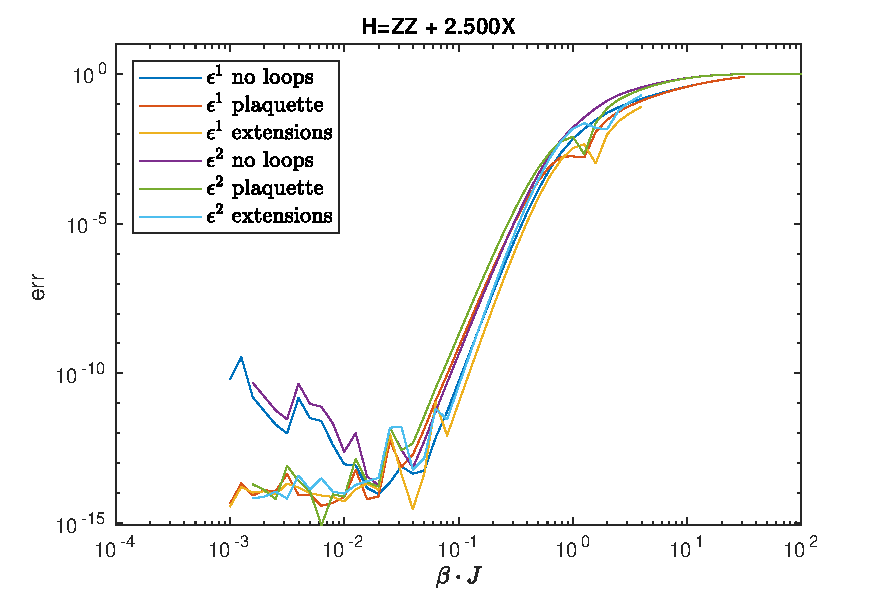
\includegraphics[width=\textwidth]{../Figuren/benchmarking/2D_Err01_t_sing.pdf}
        \end{figure}
    \end{minipage}
    \begin{minipage}{.24\textwidth}
        \begin{table}[]
            \caption{$\chi$}
            \begin{tabular}{l|l }
                no loops   & 21 \\
                loops      & 27 \\
                extensions & 43 \\
            \end{tabular}
        \end{table}
    \end{minipage}
\end{frame}

\subsection{2D Transverse Ising model}

\begin{frame}{2D: TFI}
    \begin{figure}
        \centering
        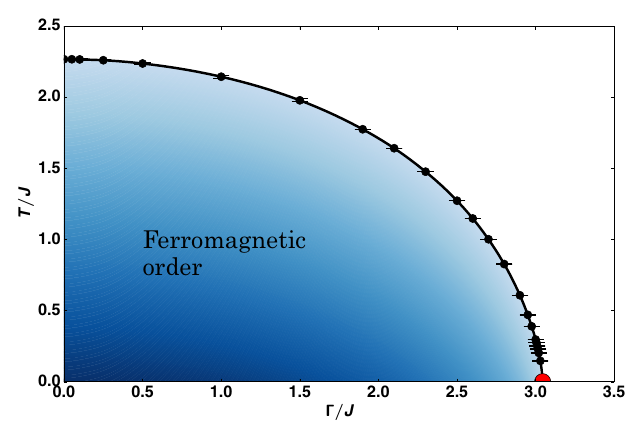
\includegraphics[width=0.75 \linewidth]{../Figuren/phsyics/2disingphase.png}
        \caption{Figure taken from \cite{Hesselmann2016}  }
    \end{figure}
\end{frame}

\begin{frame}{2D: Classical Ising}
    \begin{minipage}{.75\textwidth}
        \begin{figure}
            \center
            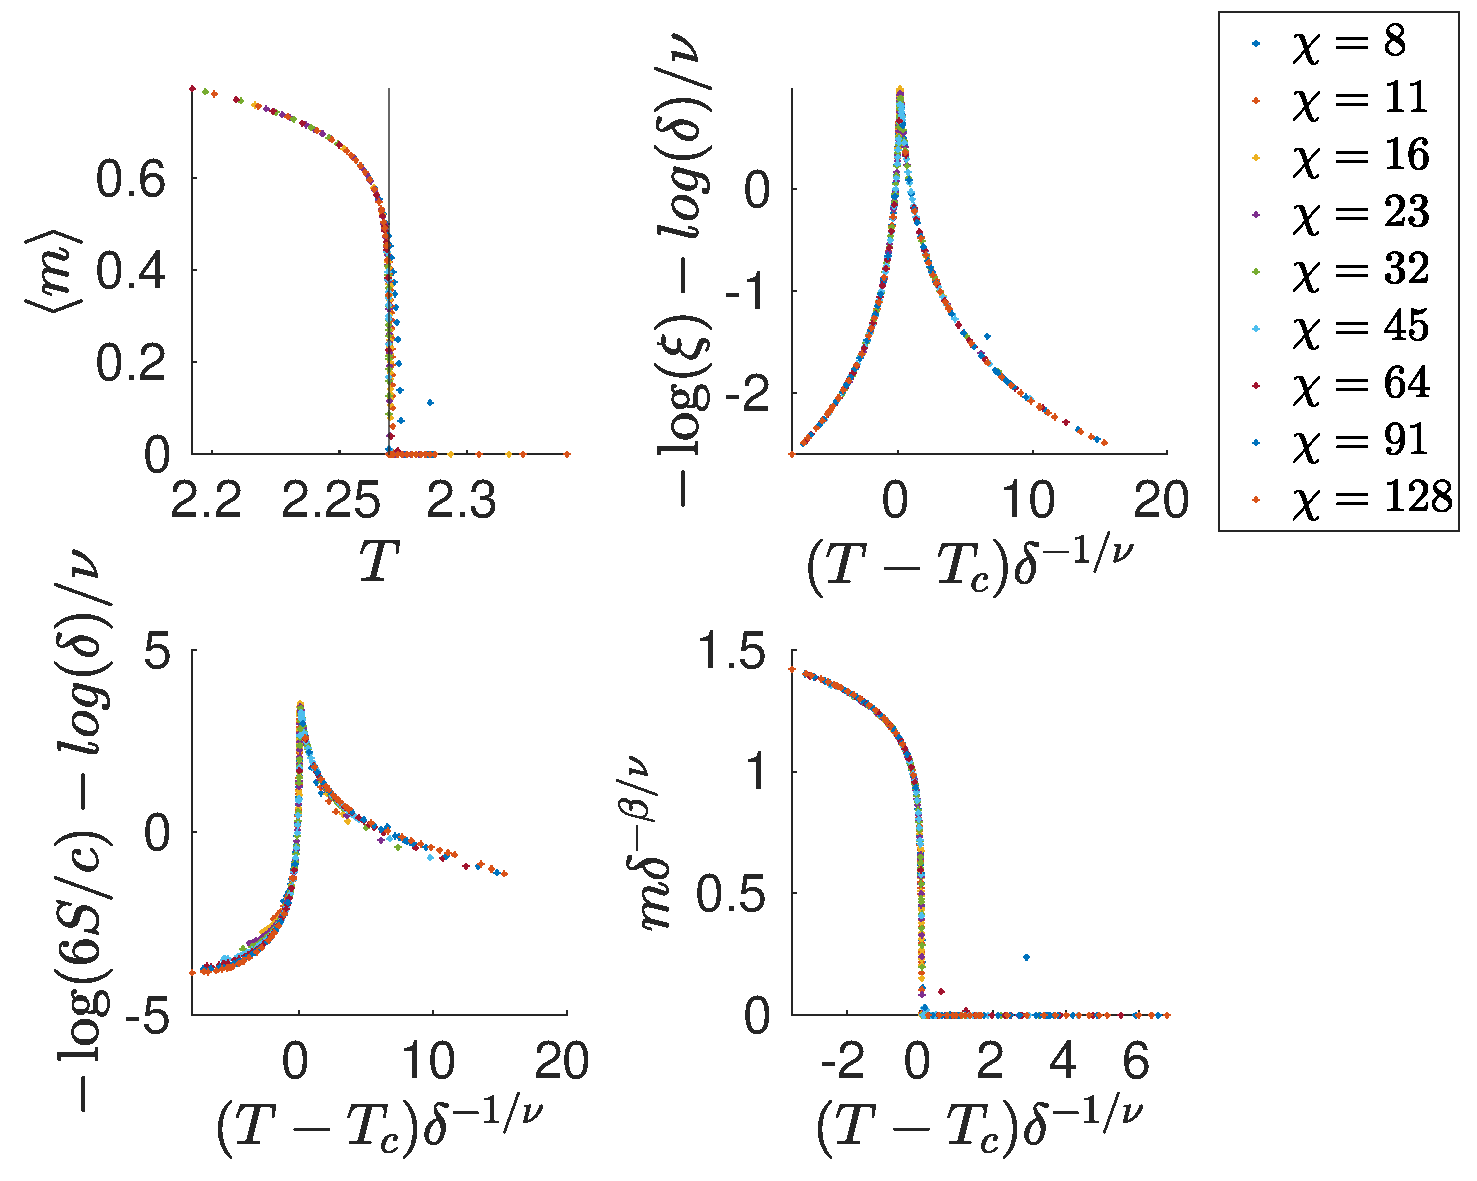
\includegraphics[height=\textheight]{../Figuren/phasediag/g0/zoomed_small.pdf}
        \end{figure}
    \end{minipage}
    \begin{minipage}{.24\textwidth}
        \begin{table}[]
            \begin{tabular}{l|l }
                      & $T_c$    \\
                \hline           \\
                Fit   & 2.691(9) \\
                Exact & 2.691853 \\

            \end{tabular}
        \end{table}

        % \begin{itemize}
        %     \item Fitted $T_c=2.691(9)$
        %     \item Exact $T_c \approx 2.69185 $
        % \end{itemize}
    \end{minipage}
\end{frame}

\begin{frame}{2D: TFI $g=2.5$}
    \begin{minipage}{.75\textwidth}
        \begin{figure}
            \center
            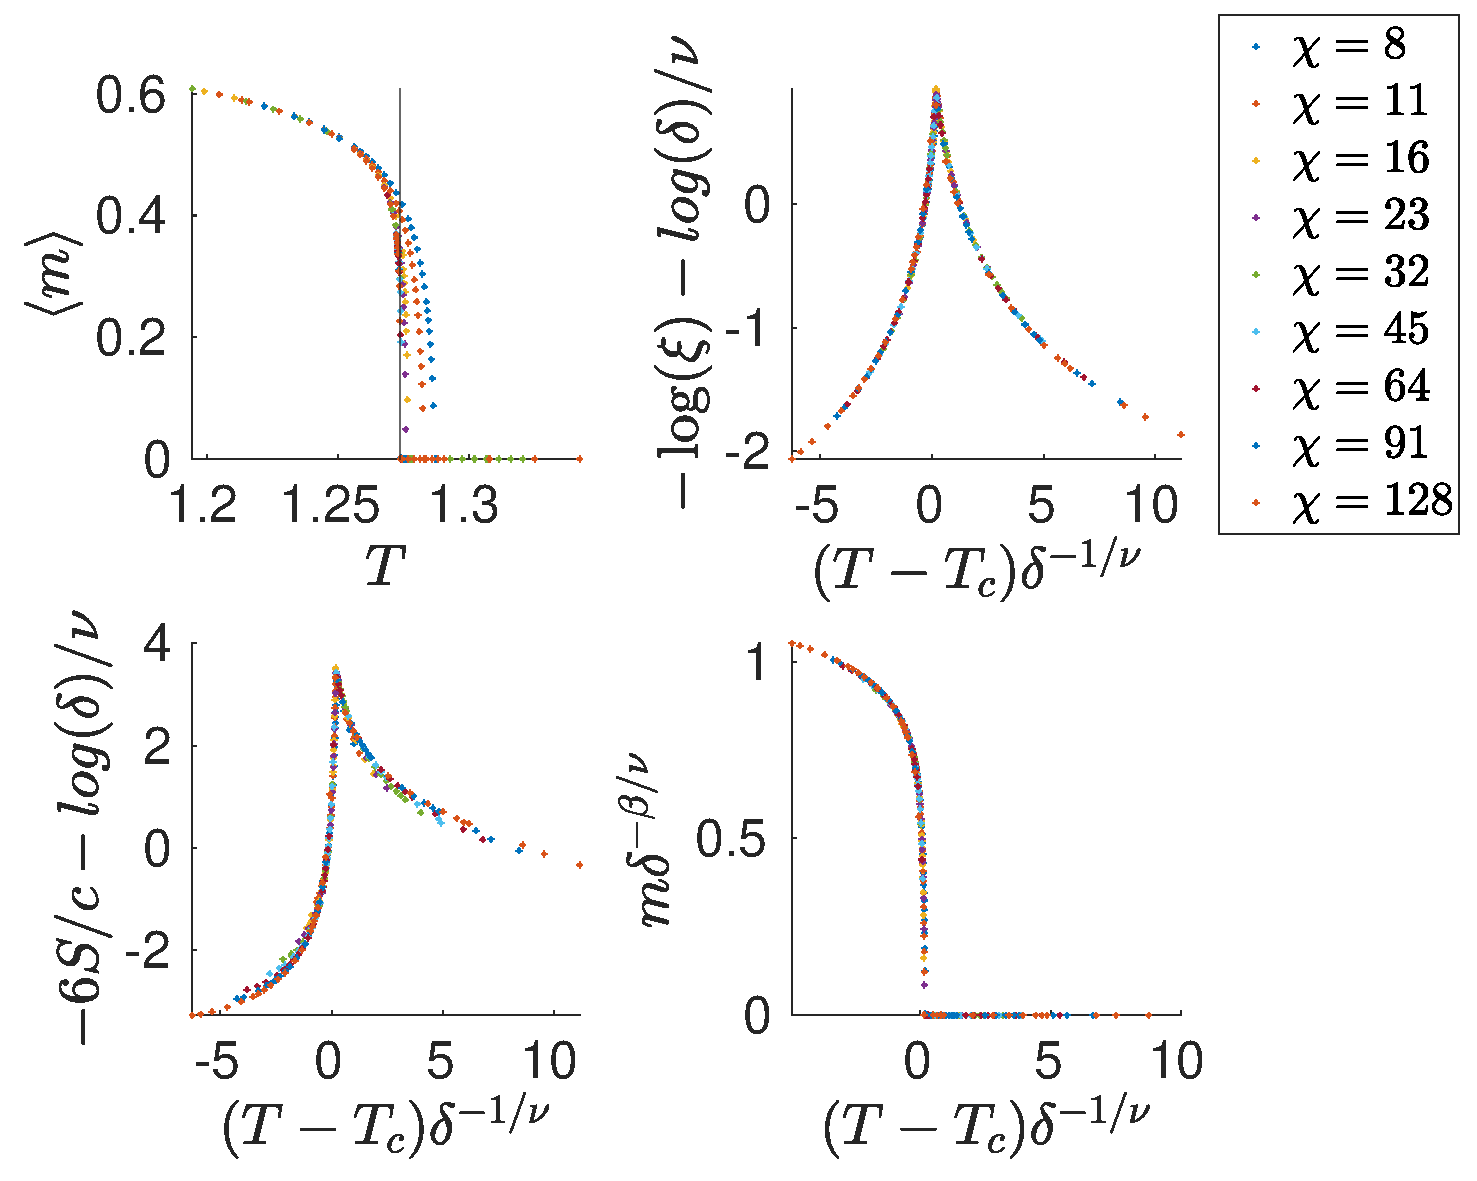
\includegraphics[height=\textheight]{../Figuren/phasediag/g25/zoomed_small.pdf}
        \end{figure}
    \end{minipage}
    \begin{minipage}{.24\textwidth}
        \begin{table}[]
            \caption{Data from  \cite{Czarnik2019} }
            \begin{tabular}{l|l }
                    & $T_c$     \\
                \hline          \\
                Fit & 1.2736(6) \\
                QMC & 1.2737(6) \\
                TN  & 1.2737(2) \\
            \end{tabular}
        \end{table}
    \end{minipage}
\end{frame}
